\chapter{Payola}
\label{ch:payola}

Quite some time ago, we decided to participate on a~large--scale software 
project focused on analyzing and visualising Linked Data. As a~result of the~project
a~completely new tool, Payola, was introduced. Since we are proposing a 
system, which could fit into the technological stack of Payola, in this chapter, 
we will get the reader familiar with the tool. Even if we  decide 
not to integrate the system we are about to propose, the Payola tool remains
a related work tool and worth describing.

Payola is an~HTML5 application oriented on a generic processing of Linked Data. 
The main goal was to come up with an~application that will eventually reduce the~software 
stack one needs to browse, analyze and visualize Linked Data. We wanted the~tool 
to compile some existing approaches and bring a~compact way for processing LD.

Upon a closer look at Section ~\ref{chap:rw}, it will become apparent that many of those tools are
immensely capable. However at a more detailed look one will see that they might have to
be chained in order to convert data into 
RDF, perform analysis over an~RDF graph and visualize those results.

Payola, on the~other hand, is a~framework developed with keeping in mind that 
the user should have no need for another tool to process their data. However, as a~
large--scale project actively being developed, it still lacks many 
features and originally offers just a~basic set of operations to enable a
\emph{generic} processing of an~arbitrary dataset.

To understand the~architecture of a possibly proposed plugin, we need to walk the reader 
through the~architecture of the~framework itself. But, to be able to understand 
the architecture of the~system it is required to familiarize oneself with its features first.

\section{Payola concepts}
In order to fully understand the~following text, let us explain some concepts 
implemented in Payola:
\begin{itemize}
  \item \emph{Data Source} --- data storage with a~defined interface like a~SPARQL endpoint.
  If we talk about a~data source, we almost always have in mind an~RDF data source.
  
  \item \emph{Analysis} --- one can look at an~analysis as an~algorithm, which 
  describes working with data from a data source in order to provide results. 
  It is a~way of specifying the data sources you want to fetch the~data from, 
  filtering them, combining them, constraining them on properties, applying 
  ontologies, etc. Also known as an analytical pipeline or an analyser.  
  
  \item \emph{Plugin} --- as Payola is a~platform, it is reasonable to expect that 
  some of the~features might get to be extended by plugins. In 
  Payola, we distinguish between two different types of plugins --- \emph{analytical plugins} and 
  \emph{visualisation plugins}. Whilst visualisation plugins are small components, 
  which take an~RDF graph as an~input, the~analytical plugins are processing 
  units, which generally transform one~input graph (or more) into another one.
  
  That includes anything from a simple forwarding of the~graph from input to output, 
  making union of two graphs, executing a~SPARQL query on the~graph to constructing 
  a~completely different graph. The new graph is created by applying in--memory
  operations defined by the~source code of the~plugin.
  
  \item \emph{Data fetcher} --- a~component, which serves to fetch data from a~data 
  source. For example, while communicating with DBPedia~\cite{dbpedia},
  a~data fetcher is needed to connect to a~SPARQL Endpoint, execute a~
  SPARQL query against it and return the~results.
\end{itemize}

\section{Payola features}
Basically, we differentiate between two types of Payola users --- anonymous and registered. 
While an~anonymous user has a~very limited accessibility as they can only 
view and explore publicly available resources a~registered user is able to 
take a full advantage of the~application.

One of the~basic features offers the~possibility of creating your own instances of a~
data source. Based on the~available data fetcher types, the~user is able to create 
his own instance. An instance is a mean where one specifies parameters of a~
concrete data fetcher. For example in the~case of a~SPARQL Endpoint data fetcher,
the user fills in the~URL of the~SPARQL Endpoint and optionally a~URI of the~named graph 
containing the~desired dataset. Having done this, the~user is able to share 
such an~instance with the~other users of Payola.
Moreover, the~user can make it 
publicly available and share an~URL of that instance, which allows any 
Internet user to browse through the~data source equally as its owner.

\subsection{Exploration mode}
On the~application dashboard is the~user presented with a~list of accessible 
resources, including data sources. After clicking on a~data source the~user is
presented with a~neighbourhood of an~\emph{initial vertex}. The choice of an~initial vertex
depends on the~implementation of the~underlying data fetcher.
Those bundled with Payola choose a~random entity from the~data source
and use it as a~starting point of a~data source exploration.

The user is also provided with his own data repository, which is created by 
Payola in the~underlying installation of the~Virtuoso~\cite{virtuoso} triplestore. Payola then eases 
the upload of an~arbitrary dataset in the~RDF/XML or TTL 
format into the~private repository. The repository may be used as a~data source in analyses.

In the~exploration mode, one can choose from a~couple of visualisation plugins. 
By default, the~results are displayed in a form of a~triple table, but the~user can 
opt to more advanced modes --- a graph visualisation and a chart visualisation
(which currently requires a~special pattern to be present in the~data). By using those 
visualizers, the~user is able to traverse from a node to a node, thus exploring the~whole 
dataset.

\subsection{Analytical mode}
In the~analytical mode, the~user is able to build a~custom data analysis. As 
stated before, an~analysis could be presented as an~algorithm, which decides 
how to process data. Moreso, in the~analysis, one is expected to specify 
where the~data have to be fetched from.

The analysis concept arises from ideas seen in projects like DERI 
Pipes~\cite{deri-pipes}, meaning, that the~user is needed to assemble a~pipeline,
which processes the~input data in a~specified way. Therefore, to enable them a 
building of an~analysis, Payola is bundled with several basic 
plugins. Generally, the~list of plugins contains as many plugins as needed
in order to simulate basic SPARQL query behaviour.

\begin{itemize}
  \item \emph{Typed} --- This plugin selects vertices of an~RDF type that is filled in
  as a~parameter called RDF Type URI from its input graph.
  
  \item \emph{Property Selection} --- the~plugin takes property URIs separated by the
  newline character as a~single parameter. It selects vertices connected
  to others using one of the~listed URIs.
  
  \item \emph{Filter} --- the~plugin lets the~user select vertices with an~attribute of
  a~particular value or property.
 
  \item \emph{Ontological Filter} --- this plugin filters the~input data so that the~
  result contains only vertices and properties defined in an~ontology specified 
  by the~given URI.
  
  \item \emph{SPARQL Query} --- a~plugin for more advanced users who are capable of 
  constructing a~custom SPARQL query. Since plugins in the~pipeline work solely with 
  graphs, the~SPARQL query should be of a CONSTRUCT type.
  
  \item \emph{Union} --- a~plugin with more than one input. As the name suggests, it takes 
  the~input graphs and unifies them into a~single one that is passed onto the~
  output.
  
  \item \emph{Join} --- the~behaviour of the~Join plugin could be a~bit tricky so it is advisible
  to take a~closer look at it in the~application's 
  user guide~\cite{payola:ug:join-plugin}. The most common case simulates the~
  behaviour of the~join statement as we know it from the~world of relational 
  databases.
  
\end{itemize}

An example of an~analysis can be seen in the~figure~\ref{fig:example-analysis}.
The goal of the~analysis is to query against DBPedia SPARQL Endpoint and 
retrieve cities with a~number of population higher than the~specified parameter. 
Those cities are then connected to the~country they belong to.

\begin{figure}
	\centering
	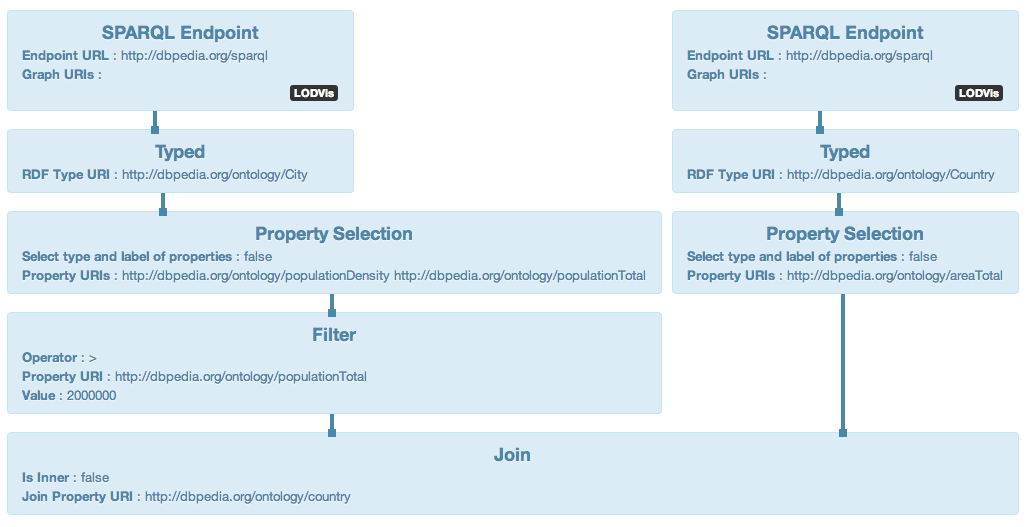
\includegraphics[width=150mm]{images/example-analysis.png}
	\caption{An example of Payola analysis}
	\label{fig:example-analysis}
\end{figure}

\subsection{Visualisations}
One would certainly like to visualize the~results of an~analysis. Therefore, 
Payola is bundled with some basic visualizer plugins. As described
in Chapter ~\ref{chap:rw}, the~Payola basic visualization 
plugins support some features suggested in the~Visualisation 
mantra~\cite{mantra}.

The bundled plugins enable the user to visualize the~results of an~analysis 
in a~couple of different ways. The basic visualisation generates a~triple 
table, while more advanced variants offer a~generic graph visualisation with a 
support of OWL ontologies. The visualizer allows the~user to customize the~
view based on an~ontology. The user can customize colours and other graphical 
features of a~rendered graph representation in respect to a~URI type defined in 
an ontology.

\subsection{Sharing}
Since Payola was designed as a~collaborative tool, it contains group 
managements and a~generic mechanism for sharing. Many types of content such as a 
data source, an analysis, a custom analytical plugin, an ontology customization for 
visualization, all can be shared with other users of the~Payola application 
installation.

Since the~description of the~tool is not the~main goal of this thesis, we will 
keep it brief and refer the reader to the~Payola User's guide~\cite{payola:ug} to learn more.

\section{Payola architecture}
The application is divided into several parts, packages, in fact. That can be 
seen in Figure~\ref{fig:packages-structure}. Since this will be useful in an upcoming
chapter about implementation, we will look at them more closely.

At first, there is the~\texttt{common} package consisted of a code, which is 
shared with all of the~other parts of the~application. Every other packages can 
access it and use the~declared code. Moreso, the~classes and objects 
in this package are automatically compiled into the~JavaScript language and are available
also on the~client--side. As an~example of a~class from the~common package, we
can name the \texttt{Graph} or \texttt{Vertex} classes, which serve as object representations
of an RDF graph or a~vertex (resource, entity). Moreover, there are traits for 
entities that are consequentially independent on a~concrete DAL implementation.

The domain package contains a~code related to the~business logic of the~
application. It solves mostly basic operations for entities, such as
\emph{add a~user into a~group} or \emph{grant a~certain privilege to a~user}.
It also contains components related to the~analytical plugins compiler. The 
compiler is executed when a~user submits their own analytical plugin via the~user 
interface. It validates and compiles the~code. If successful, the~plugin is 
loaded into the~application. Last, but not least, the~\emph{analysis evaluator} is 
present in this package. Since this is crucial, we will talk about the~evaluator
in more detail in this chapter.

The data package then wraps the~entities from the~previous packages with a
concrete implementation of DAL (Data Access Layer), which in our case is the~Squeryl
ORM framework~\cite{squeryl}.

The model package builds up a~wrapper, which encapsulates all the
business and data access logic. The goal of the~code in this package is to decouple
any presentation layer from the~application logic and data access. In fact,
all of the~existing presentation layers (web application controllers and
RPC remote objects) are built on top of this package. 

The web package contains all the~code needed to build the~web application --- 
a server side, a client--side and everything in between. It contains the~code of 
the MVC application as well as the~code of the~client--side subapplications.
It also contains the~code of visualizer plugins and an analysis editor. One of the~
most difficult and interesting features from this package is the~RPC mechanism.

The RPC mechanism was implemented in order to bridge the~gap between the~client 
side and the server side application and to hide the~XHR request from
the~developer of the~application and/or any extension. Since the~application heavily
uses the~\emph{Scala to JavaScript} component, we invested some effort into developing the~RPC 
protocol. That enables a developer to transparently call a~method on the~server from 
the client--side. 

\begin{figure}
	\centering
	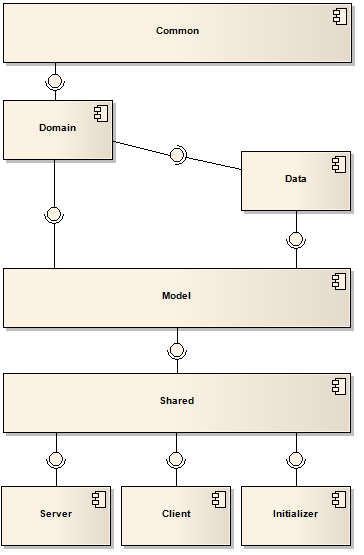
\includegraphics[width=100mm]{images/project_dependencies.png}
	\caption{Packages structure}
	\label{fig:packages-structure}
\end{figure}

To learn more about the~architecture or the implementation details, please see the~
Payola Developer's Guide~\cite{payola:dg}.

\section{Analysis evaluation}
When we are now familiar with the~parts of the~application, we may explain a~
bit more the processing and visualizing of an analytical pipeline. That is 
crucial to know before an implementation of any extension.

When an~analysis evaluation is requested, the~analysis gets \emph{validated}. We need to make
sure that the application meets some requirements, e.g. it has one 
\emph{output}, all \emph{inputs} and outputs of all the~plugins in the~analysis are \emph{bound}, etc.
If it does, the~application tries to \emph{optimize} it. Generally, executing a~plugin 
means that it is provided with an~input graph, it performs some operations and 
returns another graph. Since the~project has integrated the~Jena library~\cite{jena}, it is 
very easy to query an~in--memory representation of a~graph and return the~
results.

Let us imagine a~situation where a~user wants to select a~rather small range of 
data from a~data source. For instance, a~list of cities from DBPedia, which includes those
with a~population count higher than $2000000$ people. Without an~optimization
the evaluator would have selected all available entities from the DBPedia 
database (which is not possible anyway due to their SPARQL endpoint 
configuration). After transferring all of the~data to the~Payola server, it would have
executed a~simple SPARQL \emph{typed\&filter} query in the~memory.
However, this would be a~far cry from an~efficient solution. It would even
bring many technical difficulties, e.g. the~whole DBPedia dataset would require 
the Payola server to have a~huge amount of RAM.

That is why an~optimalization would take place in such a~situation. The original 
query which would fetch all the~data from DBPedia would be altered to include 
the constraints set by the~presence of typed and filter plugins, so that the~
data fetcher would have to fetch as less data as possible. The optimizer can 
also handle unions or joins over the~same data sources.

That gives us the~idea of how the plugins work and how they can cooperate in the~
context of analysis with optimalization. The evaluation itself is transformed 
into a~problem, which is solved by the~Scala Actors framework. For each plugin 
in the~optimized analysis, there is an~instance of an~actor. The actor waits 
until all of~the~inputs of the~corresponding plugin have been provided with the~
input data from its predecessor. When inputs are bound with input data, the~
executive part of the~plugin is performed. That could be anything from 
executing a~SPARQL query to finding the~shortest path between two nodes in a~
specified graph. The only constraint is that the~result of the~plugin execution 
needs to be also a~graph.

As the~last plugin (with no bound successor on its output) gets evaluated, the~
analysis is done. The results are sent via RPC (while being serialized into JSON) 
to the~client--side and visualized by the~basic visualisation -- the~triple 
table. The user is then able to switch to another visualisation. The JSON 
representation of the~resulting graph is stored in the~memory of the~user's web 
browser and every visualizer, which is activated by the~user accesses the~
in--memory representation and renders whatever it needs into a~given canvas.

That is a~brief description of the~evaluation process. It offers an insight
to what happens of in the~background. Later, we will learn how this affects 
the implementation of the~proposed system.

\section{Technological stack}
In order to deliver an~application, which is easy to use and does not require 
the user to install it on a~client machine, Payola is being developed as a~web
application. Since it is assumed that Linked Data community is consisted of
rather advanced computer users with modern web browsers installed, the~application 
takes advantage of a~variety of modern technologies, like HTML5 (specifically
canvas element) and CSS3.

In order to bring a~basic level of compatibility with existing applications from 
the LOD2 stack, it was decided that it has to run on the~JVM platform. The 
Scala programming language was chosen as a~main implementation language of the~
whole application. Since the~team of the~project wanted to avoid a code repeating 
while keeping in mind the~DRY programming paradigm, one of the~members 
introduced his own version of Scala to JavaScript compiler~\cite{s2js}. Therefore, even the~
client--side code of the~application is written in the~Scala programming language 
and many parts of the~code are shared between the~client--side and the~server 
side.

There were many different advantages to choosing the~Scala programming language, 
for example the~presence of the~Scala Actors framework, which fits into the~
analysis evaluation problem.

The application utilizes the~following libraries and technologies:
\begin{itemize}
  \item \emph{Play Framework 2.0} --- a~web application MVC framework completely written 
  in the~Scala programming language.
  \item \emph{SBT} --- build tool for Scala projects.
  \item \emph{jQuery} --- JavaScript library used mainly for solving crossbrowser 
  differences.
  \item \emph{Squeryl} --- Scala ORM framework used in DAL.
  \item \emph{Apache Jena} --- well known Java RDF library.
  \item \emph{Twitter Bootstrap} --- library for building an~eye-catching user 
  interface.
  \item \emph{Ace} --- JavaScript editor for programming languages.
  \item \emph{Flot} --- JavaScript chart library.
\end{itemize}

